% Data map for the README: how the tables returned by ausPH link together.
% Build from the package root:
%   cd data-raw && pdflatex data_map.tex
%   sips -s format png -Z 2400 data_map.pdf --out ../man/figures/data_map.png
%
% Solid arrows join on an identifier; dashed arrows join on a name or code,
% which needs care (see the notes on the diagram).
\documentclass[border=10pt]{standalone}
\usepackage{tikz}
\usetikzlibrary{positioning, shapes.multipart, arrows.meta, calc}
\begin{document}
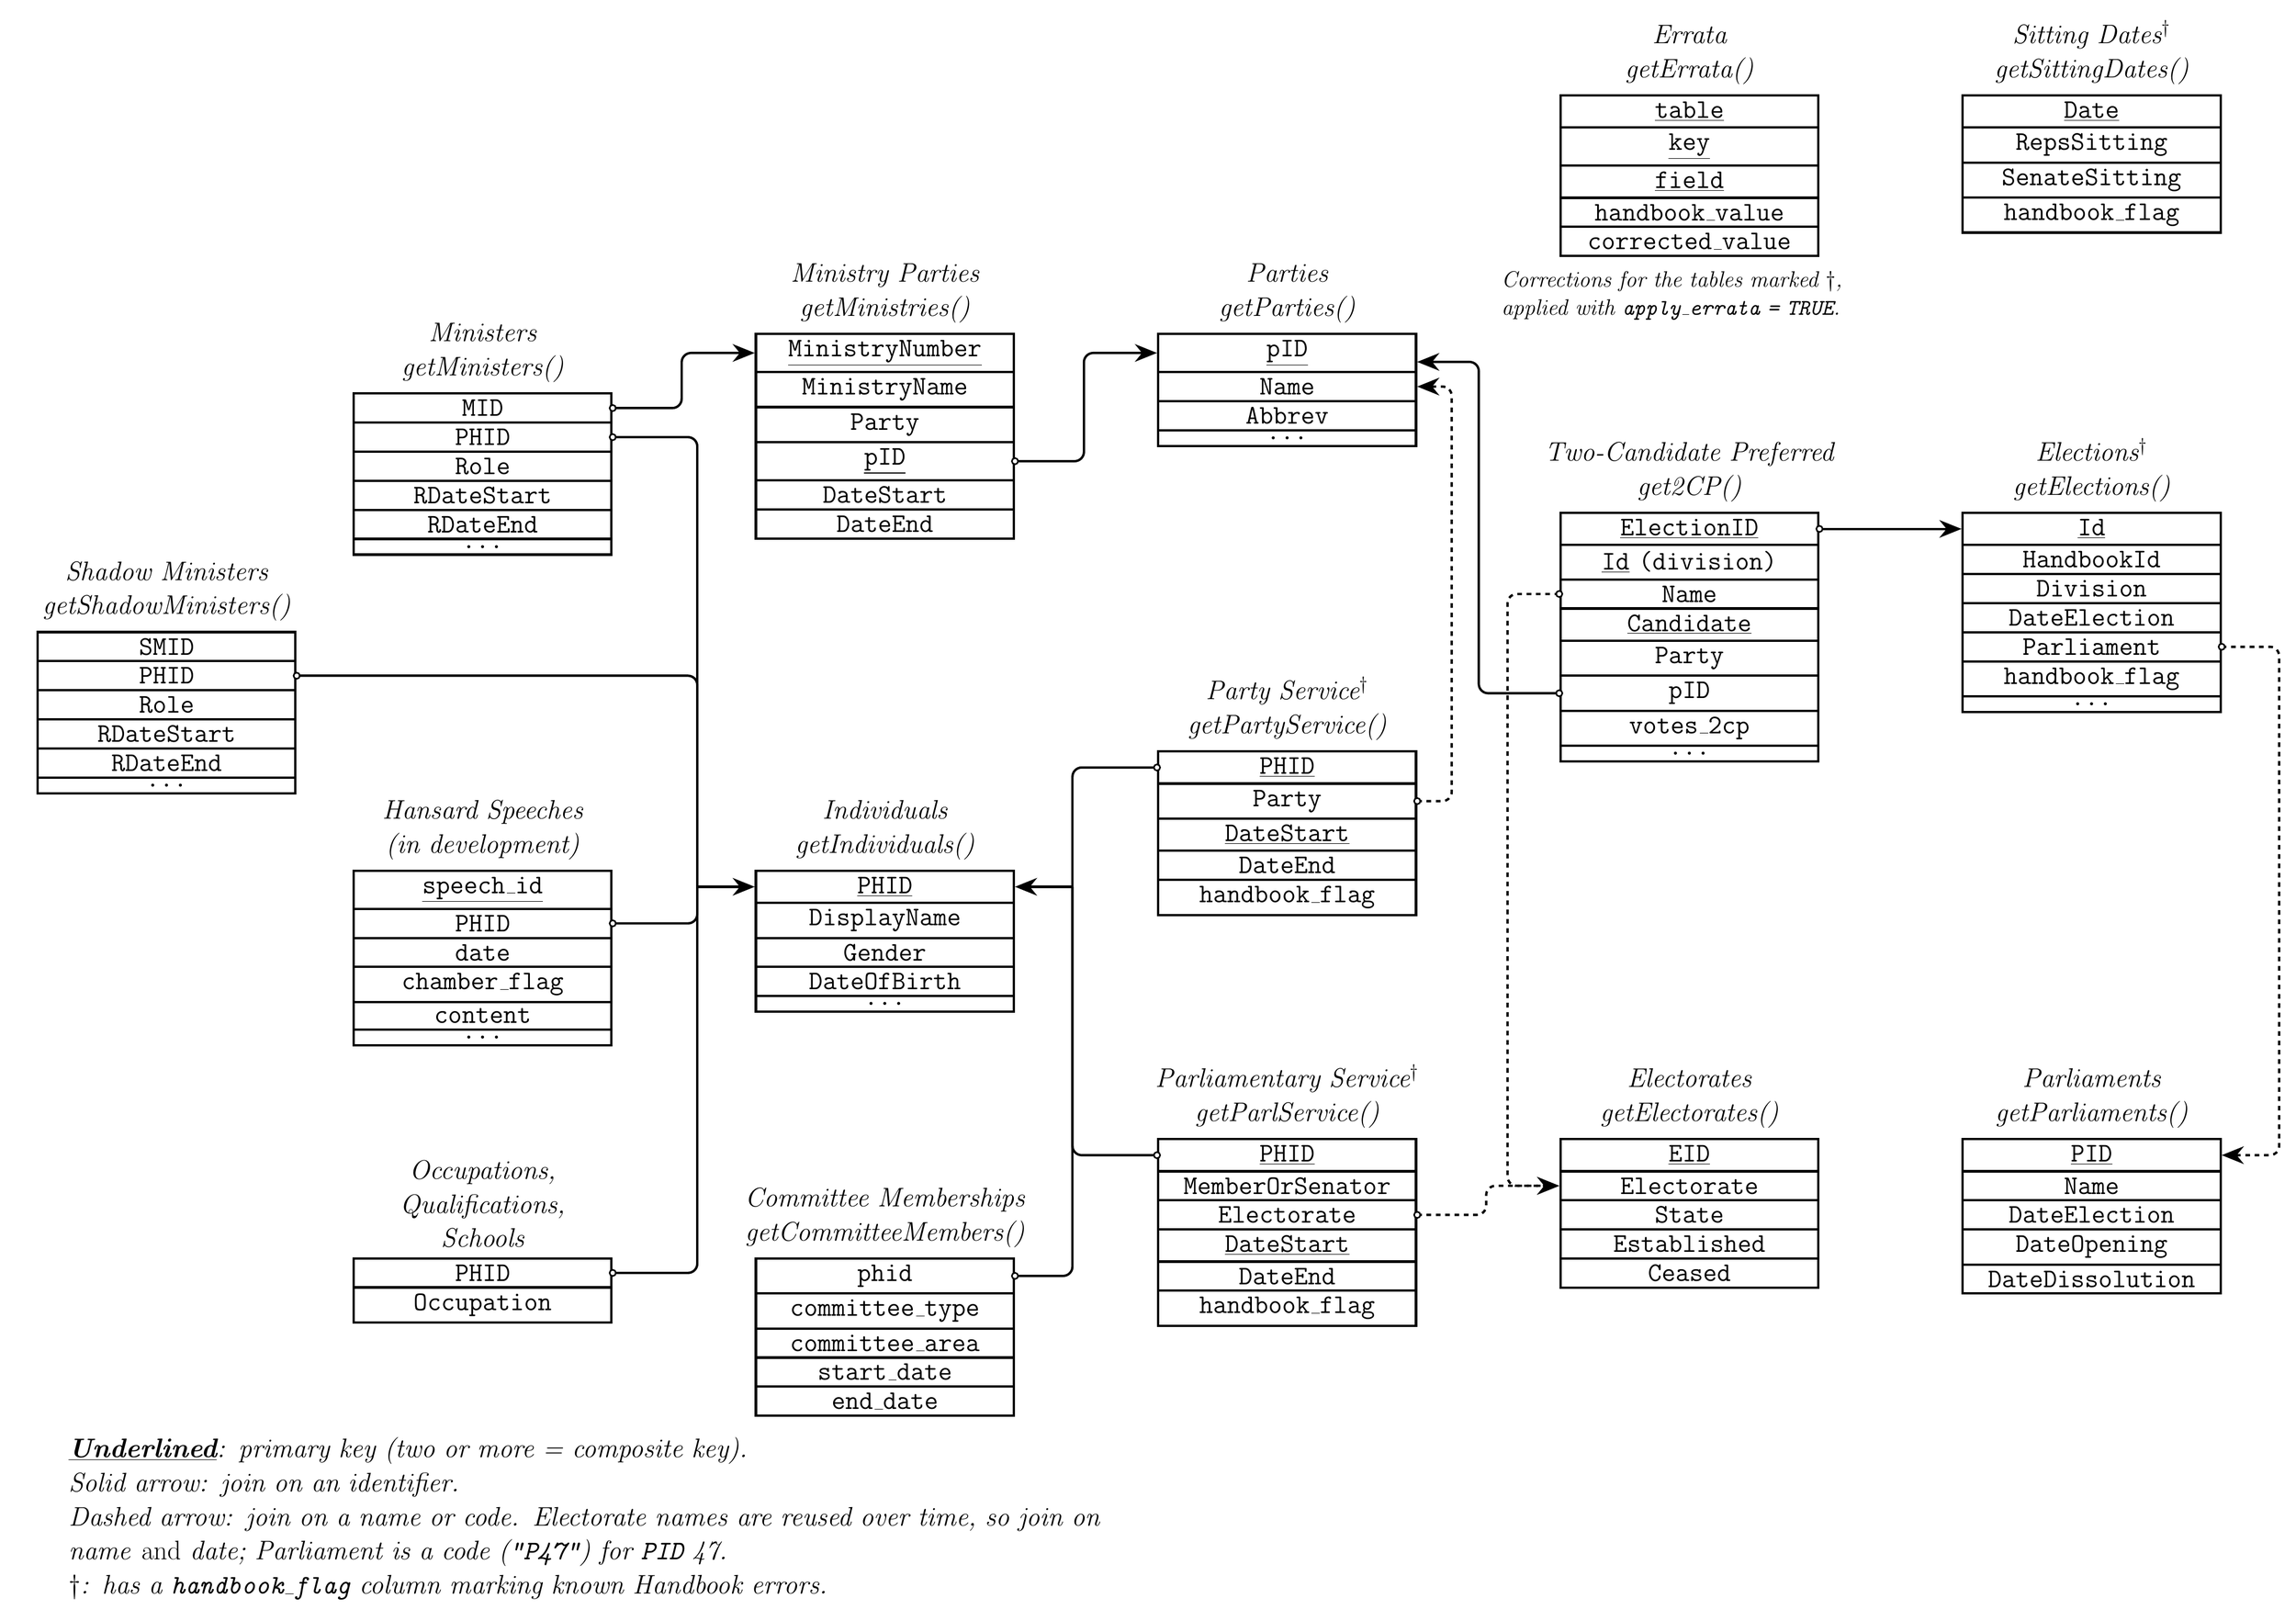
\begin{tikzpicture}[x=1.3cm, y=1.35cm,
    table/.style={
        rectangle split,
        rectangle split parts=#1,
        draw,
        line width=1.5pt,
        text width=5.6cm,
        align=center,
        font=\LARGE\ttfamily,
        fill=white,
        anchor=north
    },
    header/.style={
        font=\LARGE\itshape,
        text width=6.6cm,
        align=center,
        anchor=south
    },
    arrow/.style={
        ->,
        >={Stealth[length=5mm, width=4mm]},
        line width=1.5pt,
        rounded corners=6pt
    },
    namelink/.style={
        arrow,
        dashed
    },
    fk_dot/.style={
        circle,
        draw,
        line width=1pt,
        fill=white,
        minimum size=4pt,
        inner sep=0pt
    },
    note/.style={
        font=\Large\itshape,
        text width=7.5cm,
        align=left
    }
]

% PK = underlined (two underlined fields = composite key). $\dagger$ = has a
% handbook_flag column and can take apply_errata = TRUE.

% ===== people (centre) =====

\node[header] (individuals-header) at (0,0) {Individuals\\getIndividuals()};
\node[table=5, below=0.1cm of individuals-header.south] (individuals) {
    \textbf{\underline{PHID}}
    \nodepart{two} DisplayName
    \nodepart{three} Gender
    \nodepart{four} DateOfBirth
    \nodepart{five} ...
};

\node[header] (speeches-header) at (-7,0) {Hansard Speeches\\(in development)};
\node[table=6, below=0.1cm of speeches-header.south] (speeches) {
    \textbf{\underline{speech\_id}}
    \nodepart{two} PHID
    \nodepart{three} date
    \nodepart{four} chamber\_flag
    \nodepart{five} content
    \nodepart{six} ...
};

\node[header] (occupations-header) at (-7,-6.5) {Occupations, Qualifications,\\Schools};
\node[table=2, below=0.1cm of occupations-header.south] (occupations) {
    PHID
    \nodepart{two} Occupation
};

\node[header] (committee-header) at (0,-6.5) {Committee Memberships\\getCommitteeMembers()};
\node[table=5, below=0.1cm of committee-header.south] (committee) {
    phid
    \nodepart{two} committee\_type
    \nodepart{three} committee\_area
    \nodepart{four} start\_date
    \nodepart{five} end\_date
};

% ===== government (top) =====

\node[header] (ministers-header) at (-7,8) {Ministers\\getMinisters()};
\node[table=6, below=0.1cm of ministers-header.south] (ministers) {
    MID
    \nodepart{two} PHID
    \nodepart{three} Role
    \nodepart{four} RDateStart
    \nodepart{five} RDateEnd
    \nodepart{six} ...
};

\node[header] (shadow-header) at (-12.5,4) {Shadow Ministers\\getShadowMinisters()};
\node[table=6, below=0.1cm of shadow-header.south] (shadow) {
    SMID
    \nodepart{two} PHID
    \nodepart{three} Role
    \nodepart{four} RDateStart
    \nodepart{five} RDateEnd
    \nodepart{six} ...
};

\node[header] (ministries-header) at (0,9) {Ministry Parties\\getMinistries()};
\node[table=6, below=0.1cm of ministries-header.south] (ministries) {
    \textbf{\underline{MinistryNumber}}
    \nodepart{two} MinistryName
    \nodepart{three} Party
    \nodepart{four} \textbf{\underline{pID}}
    \nodepart{five} DateStart
    \nodepart{six} DateEnd
};

\node[header] (parties-header) at (7,9) {Parties\\getParties()};
\node[table=4, below=0.1cm of parties-header.south] (parties) {
    \textbf{\underline{pID}}
    \nodepart{two} Name
    \nodepart{three} Abbrev
    \nodepart{four} ...
};

% ===== service (right of centre) =====

\node[header] (party-header) at (7,2) {Party Service$^\dagger$\\getPartyService()};
\node[table=5, below=0.1cm of party-header.south] (party) {
    \textbf{\underline{PHID}}
    \nodepart{two} Party
    \nodepart{three} \textbf{\underline{DateStart}}
    \nodepart{four} DateEnd
    \nodepart{five} handbook\_flag
};

\node[header] (parlservice-header) at (7,-4.5) {Parliamentary Service$^\dagger$\\getParlService()};
\node[table=6, below=0.1cm of parlservice-header.south] (parlservice) {
    \textbf{\underline{PHID}}
    \nodepart{two} MemberOrSenator
    \nodepart{three} Electorate
    \nodepart{four} \textbf{\underline{DateStart}}
    \nodepart{five} DateEnd
    \nodepart{six} handbook\_flag
};

% ===== elections (right) =====

\node[header] (2cp-header) at (14,6) {Two-Candidate Preferred\\get2CP()};
\node[table=8, below=0.1cm of 2cp-header.south] (2cp) {
    \textbf{\underline{ElectionID}}
    \nodepart{two} \textbf{\underline{Id}} (division)
    \nodepart{three} Name
    \nodepart{four} \textbf{\underline{Candidate}}
    \nodepart{five} Party
    \nodepart{six} pID
    \nodepart{seven} votes\_2cp
    \nodepart{eight} ...
};

\node[header] (electorates-header) at (14,-4.5) {Electorates\\getElectorates()};
\node[table=5, below=0.1cm of electorates-header.south] (electorates) {
    \textbf{\underline{EID}}
    \nodepart{two} Electorate
    \nodepart{three} State
    \nodepart{four} Established
    \nodepart{five} Ceased
};

\node[header] (elections-header) at (21,6) {Elections$^\dagger$\\getElections()};
\node[table=7, below=0.1cm of elections-header.south] (elections) {
    \textbf{\underline{Id}}
    \nodepart{two} HandbookId
    \nodepart{three} Division
    \nodepart{four} DateElection
    \nodepart{five} Parliament
    \nodepart{six} handbook\_flag
    \nodepart{seven} ...
};

\node[header] (parliaments-header) at (21,-4.5) {Parliaments\\getParliaments()};
\node[table=5, below=0.1cm of parliaments-header.south] (parliaments) {
    \textbf{\underline{PID}}
    \nodepart{two} Name
    \nodepart{three} DateElection
    \nodepart{four} DateOpening
    \nodepart{five} DateDissolution
};

% ===== standalone tables =====

\node[header] (sitting-header) at (21,13) {Sitting Dates$^\dagger$\\getSittingDates()};
\node[table=4, below=0.1cm of sitting-header.south] (sitting) {
    \textbf{\underline{Date}}
    \nodepart{two} RepsSitting
    \nodepart{three} SenateSitting
    \nodepart{four} handbook\_flag
};

\node[header] (errata-header) at (14,13) {Errata\\getErrata()};
\node[table=5, below=0.1cm of errata-header.south] (errata) {
    \textbf{\underline{table}}
    \nodepart{two} \textbf{\underline{key}}
    \nodepart{three} \textbf{\underline{field}}
    \nodepart{four} handbook\_value
    \nodepart{five} corrected\_value
};
\node[note, text width=8.5cm, below=0.2cm of errata.south] {Corrections for the tables marked $\dagger$, applied with \texttt{apply\_errata = TRUE}.};

% ===== legend =====

\node[note, font=\LARGE\itshape, anchor=north west, text width=24cm] (legend) at (-14.3,-9.5) {
    \textbf{\underline{Underlined}}: primary key (two or more = composite key).\\
    Solid arrow: join on an identifier.\\
    Dashed arrow: join on a name or code. Electorate names are reused over
    time, so join on name \emph{and} date; Parliament is a code (\texttt{"P47"})
    for \texttt{PID} 47.\\
    $\dagger$: has a \texttt{handbook\_flag} column marking known Handbook errors.
};

% ===== PHID links to Individuals =====
% links from each side run into one line, which meets Individuals.PHID

\coordinate (bus-left) at ($(individuals.text west)+(-1.0,0)$);
\coordinate (bus-right) at ($(individuals.text east)+(1.0,0)$);

\draw[line width=1.5pt, rounded corners=6pt] (shadow.two east) -| (bus-left);
\draw[line width=1.5pt, rounded corners=6pt] (ministers.two east) -| (bus-left);
\draw[line width=1.5pt, rounded corners=6pt] (speeches.two east) -| (bus-left);
\draw[line width=1.5pt, rounded corners=6pt] (occupations.text east) -| (bus-left);
\draw[arrow] (bus-left) -- (individuals.text west);
\foreach \fk in {shadow.two east, ministers.two east, speeches.two east, occupations.text east}
    \node[fk_dot] at (\fk) {};

\draw[line width=1.5pt, rounded corners=6pt] (party.text west) -| (bus-right);
\draw[line width=1.5pt, rounded corners=6pt] (parlservice.text west) -| (bus-right);
\draw[line width=1.5pt, rounded corners=6pt] (committee.text east) -| (bus-right);
\draw[arrow] (bus-right) -- (individuals.text east);
\foreach \fk in {party.text west, parlservice.text west, committee.text east}
    \node[fk_dot] at (\fk) {};


% ===== ministries and parties =====

\draw[arrow] (ministers.text east) -- ++(1.2,0) |- (ministries.text west);
\node[fk_dot] at (ministers.text east) {};

\draw[arrow] (ministries.four east) -- ++(1.2,0) |- (parties.text west);
\node[fk_dot] at (ministries.four east) {};

\draw[arrow] (2cp.six west) -- ++(-1.4,0) |- ($(parties.text east)+(0,-0.15)$);
\node[fk_dot] at (2cp.six west) {};

\draw[namelink] (party.two east) -- ++(0.6,0) |- (parties.two east);
\node[fk_dot] at (party.two east) {};

% ===== elections =====

\draw[arrow] (2cp.text east) -- (elections.text west);
\node[fk_dot] at (2cp.text east) {};

\draw[namelink] (elections.five east) -- ++(1,0) |- (parliaments.text east);
\node[fk_dot] at (elections.five east) {};

\draw[namelink] (2cp.three west) -- ++(-0.9,0) |- (electorates.two west);
\node[fk_dot] at (2cp.three west) {};

\draw[namelink] (parlservice.three east) -- ++(1.2,0) |- (electorates.two west);
\node[fk_dot] at (parlservice.three east) {};

\end{tikzpicture}
\end{document}
